\documentclass[11pt]{article}
\usepackage[top=1.5in, bottom=1.5in, left=1in, right=1in]{geometry}
\usepackage{adjustbox}
\usepackage{graphicx}

\begin{document}

%Titlepage
\begin{titlepage}
\title{\textbf{EPO-2 "Smart Robot Challenge"} \\\textbf{Plan van Aanpak}}
\author{Groep D-2}
\date{\today}
\clearpage\maketitle
\thispagestyle{empty}
\end{titlepage}

%Table of Contents
\thispagestyle{empty}
\setcounter{page}{0}
\tableofcontents
\clearpage

%Sections
\newpage
\section{Achtergronden}
De opdrachtgever en -nemer voor dit project is de TU Delft met als studierichting Electrical Engineering. Dit project is om educatieve doeleinden opgestart en wordt door iedereen uit het eerstje jaar uitgevoerd, dit wordt gedaan in groepen van zes tot acht personen.  Aan de hand van dit project wordt de opgedane kennis uit de hoor- en werkcolleges in de praktijk toegepast. Benodigde kennis die niet tijden colleges worden behandeld, zullen in zo genaamde just-in-time trainingen en tutorials uitgelegd worden, deze zullen worden uitgevoerd of op de drebbelweg  5 of in het gebouw van Technische Natuurkunde.
Het doel van het project is het ontwerpen van een autonoom mijndetecterende robot. Het is de bedoeling dat we deze robot in een vooraf bepaal veld laten rijden en daar met een zelf ontworpen sensor de mijnen in kaart weten brengen, om deze vervolgens te ontwijken. De ”Smart Robot Challange” wordt aan het einde van kwartaal vier afgesloten met een wedstrijd.

\section{Projectresultaat}
Er moet als groep een autonoom mijndetecterende robot worden ontworpen. Door middel van een vooraf bepaalde kaart en een zelf ontworpen sensor, moet de robot de mijnen ontwijken en ook in kaart brengen. Voor de robot zelden enkele technische eisen\footnote{Ir. A.C. de Graaf, Dr. ir. M.A.P. Pertijs, Dr. M. Bartek, \textit{Semesterboek 2 Smart Robot Challenge}. 2012-2013, TU Delft}:

\begin{itemize}
\item De robot past in een fictieve box (is niet groter dan) 30 cm x 25 cm x 20 cm;

\item Het gewicht is maximaal 1 kg;

\item De aandrijving is gerealiseerd m.b.v. elektromotoren en een batterij. Behalve
batterij is er op de robot geen andere energiebron aanwezig.

\item De robotaansturing kan gerealiseerd worden alleen via de beschikbare Basys2 ontwikkelbord met Spartan-3 FPGA chip, twee XBee modules en een besturingsprogramma op een laptop/PC geschreven in programmeertaal C. De configuratie van
de FPGA-chip kan geschieden alleen via een in-VHDL-geschreven broncode.

\item Het besturingsprogramma moet zo geschreven zijn, dat het door de gebruiker niet
mogelijk is de posities van de obstakels of de vrije wegsegmenten op het wedstrijdveld in te voeren.

\item De robot moet zo geconstrueerd zijn, dat deze geen schade of markeringen aan het
wedstrijdveld aanbrengt.
\end{itemize}

\newpage
\section{Projectactiviteiten}
\subsection{Opamps (meetrapport)}
De tweetallen die aan dit onderwerp werken:
\begin{enumerate}
\item Luc Does, Tijmen Witte;
\item Erwin de Haan, Robin Hes;
\item Joris Blom, Chy Lau;
\end{enumerate}
In dit onderdeel wordt de werking van de relaxatie oscillator geanalyseerd. Per tweetal moet een rapport worden ingeleverd bij de tutor. Het rapport mag maximaal 5 pagina's omvatten. 

\subsection{Ontwerprapport met systeemspecificaties en routeplanner}
De deelgroepen die zich op de volgende onderdelen concentreren:
\begin{itemize}
\item Systeemspecificaties: Joris Blom, Luc Does, Chy Lau, Tijmen Witte;
\item Routeplanner in C: Erwin de Haan, Robin Hes;
\end{itemize}
In het verslag moeten minimaal de volgende punten worden besproken: systeemspecificaties en routeplanner in C. Dit verslag wordt geëvalueerd door de tutor en is 10\% van de eindcijfer.

\subsection{Zelfevaluatierapport Q3}
Ieder groepslid moet een zelfevaluatierapport van 1 A-4 schrijven voor kwartaal 3. De volgende punten moeten in het verslag verwerkt worden:
\begin{itemize}
\item Wat je hebt geleerd in EPO-2 tijdens het 3e kwartaal;
\item Waren de activiteiten nuttig?;
\item Je eigen contributie aan het projectresultaat;
\item Wat was goed en wat moet er nog verbeterd worden?;
\item Overige opmerkingen;
\end{itemize}
Dit rapport wordt gebruikt als input voor het gesprek met de tutor. 


\subsection{Niet-Lineaire Schakelingen}
Deelgroepen die aan dit onderdeel werken:
\begin{itemize}
\item Opdracht 1: Joris Blom, Chy Lau, Tijmen Witte;
\item Opdracht 2: Luc Does, Erwin de Haan, Robin Hes;
\end{itemize}
Twee opdrachten over niet-lineaire schakelingen worden uitgewerkt. Over de opdrachten moet een verslag worden geschreven. Bovendien moeten ze aan de groepsleden gepresenteerd worden, zodat alle teamleden de kennis hebben van dit onderdeel.

\subsection{Ontwerprapport (draft)}
Er moet minimaal 1 kwantitatieve meting aan de robot worden verwerkt in het verslag. Voorbeelden daarvan zijn:
\begin{itemize}
\item Power consumptie van de robot; Luc Does, Erwin de Haan, Tijmen Witte
\item Invloed van de batterij spanning op de snelheid van de robot; Joris Blom, Chy Lau
\item Prestatie van de mijndetector; Erwin de Haan, Robin Hes, Tijmen Witte
\item Pulsbreedte gebruikt voor de servomotor; Joris Blom, Robin Hes, Chy Lau 
\end{itemize}

\subsection{Mijnontwijkende robot (ontwerprapport)}
Samenvoegen wordt gedaan door: Robin Hes;
\\Hierin worden alle onderdelen samengevoegd tot een vollledig verslag. 

\subsection{Poster}
Groepsleden die aan dit onderdeel werken zijn: Erwin de Haan, Chy Lau;
\\De poster van A-3 formaat moet gerelateerd zijn aan een van de subsystemen, bijvoorbeeld: mijndetector circuit, route optimalisatie, etc. 

\newpage
\section{Tussenresultaat}
Aan het eind van de 3de kwartaal moet de projectgroep de volgende doelen (robot mini-challenges) bereiken\footnote{\textit{TU Delft Blackboard}. \texttt{https://blackboard.tudelft.nl}, Smart Robot Challenge-Resources}:

\begin{itemize}
\item De robot kan autonoom een zwarte lijn volgen (mini-challenge 1);
\item De robot kan vanaf de laptop draadloos m.b.v. de ZigBee modules worden aangestuurd (mini-challenge 2).
\item Een goedwerkende C-programma voor een routeplanner in Challenges A en B.
\end{itemize}

\section{Kwaliteit}
Door middel van het toepassen van kennis en vaardigheden die in het 1ste en 2de semester zijn verkregen, is het doel van het project om de robot zo snel mogelijk van punt A naar punt B te laten gaan en de tussenliggende mijnen detecteert. Om de kwaliteit te waarborgen, wordt alles eerst gesimuleerd, zodat kan worden vastgesteld of alles functioneert. Voor het simuleren wordt een C-compiler en een VHDL-compiler gebruikt.\\
\indent Er moeten meer verslagen worden ingeleverd voor EPO-2 t.o.v. EPO-1. De verslagen zullen voornamelijk geschreven worden in \LaTeX. Het programma zal ons minder problemen opleveren dan Word bij het samenvoegen van verslagen of individuele stukken.\\
\indent Om fouten nog verder te minimaliseren, kan bij twijfel vragen worden gesteld aan de tutor en/of studentassistenten. Bovendien wordt individueel een logboek bijgehouden om eventuele onzekerheden te controleren. 

\newpage
\section{Planning}
\begin{adjustbox}{width=\textwidth,totalheight=\textheight,keepaspectratio}

\begin{tabular}{|c|p{10cm}|p{8cm}|}
\hline 
\multicolumn{3}{|c|}{\textbf{Algemene Planning}} \\ 
\hline 
\textbf{Middag} & \textbf{Activiteiten} & \textbf{Deadline} \\ 
\hline 
3.1.1 & Safety, Xilinx ISE Tutorial, Routeplanner in C & • \\ 
\hline 
3.1.2 & Routeplanner in C & Presentatie Safety \\ 
\hline 
3.2.1 & Informatievaardigheden, initieel projectplan & • \\ 
\hline 
3.2.2 & Measuring science 1 & • \\ 
\hline 
3.3.1 & Basistraining Digitale Systemen 1\&2 & Routeplanner in C, Plan van Aanpak 

(rapport en presentatie) \\ 
\hline 
3.3.2 & Basistraining Digitale Systemen 1\&2 & Robot als afstandmeter (meetrapport) 

(1 rapport per projectgroep)\\ 
\hline 
3.4.1 & Training Digitale Systemen: Inleiding VHDL, top-level beschrijving & JIT: DS1 en 2 (individueel)\\ 
\hline 
3.4.2 & Training Digitale Systemen: Tijdbasis & • \\ 
\hline 
3.5.1 & Training DS: FSM ontwerpen, inbutbuffer en robotaansturing & • \\ 
\hline 
3.5.2 & Digitale systemen - UART / ZigBee & • \\ 
\hline 
3.6.1 & JIT: Opamps & • \\ 
\hline 
3.6.2 & VHDL-code om de robot zwarte lijn te laten volgen, draadloze communicatie tussen laptop en robot m.b.v. XBee modules & Opamps (meetrapport) (groepen van 2 pers.)\\ 
\hline 
3.7.1 & Als de robot de zwarte lijn kan worden, dan verder met XBee modules & • \\ 
\hline 
3.7.2 & Idem dito & Robot challenges, Ontwerprapport, Zelfevaluatierapport Q3 (individueel)\\ 
\hline
4.1.1 & JIT; SPICE tutorial (gebruik maken pdf en lineare circuit boek) & Aflaten tekenen volgende opdrachten uit SPICE 5.111 en 5.114 (blz 246), 7.87 en 7.91(blz 370,371), 8.123 en 8.128(blz 452 en 453) 

(projectgroep)
 \\
\hline
4.1.2 & JIT; niet lineaire schakelingen & • \\
\hline
4.2.1 & Vrij & 1 van de 2 opdrachten (zie JIT; niet lineaire schakelingen)
(groepen van 2 pers.)
 \\
\hline
4.2.2 & JIT:Capacitieve sensoren (in TNW) & • \\
\hline
4.3.1 & Vrije projectmiddag (eigen invulling) & • \\
\hline
4.3.2 & JIT: Inductieve sensoren (in TNW) & • \\
\hline
4.4.1 & Meten van het verbruik van de robot & • \\
\hline
4.4.2 & Uitloop en beginnen met het bepalen van de invloed van de batterij op de snelheid & • \\
\hline
4.5.1 & De gevoeligheid van de sensoren meten en aanpassen  & • \\
\hline
4.5.2 & Uitloop van eerdere opdrachten & • \\
\hline
4.6.1 & Impuls breedte van de servo motoren meten en eventueel aanpassen & Ontwerprapport (projectgroep)
 \\
\hline
4.6.2 & Het hele systeem testen als geheel & Mijnontwijkende robot (ontwerprapport) 

(projectgroep)
\\
\hline
4.7.1 & Eventuele aanpassingen maken waar nodig & • \\
\hline
4.7.2 & Laatste controle, eventueel verbeteringen aanbrengen waar nodig & • \\
\hline
4.8 & Symposium/robot challenges en eindverdediging. & Alles af! \\
\hline
\end{tabular}

\end{adjustbox}
 

\newpage
\section{Projectorganisatie}
\textbf{Groepsleden:}\\ 
Tijmen Witte\\ 
Luc Does\\ 
Erwin de Haan\\ 
Robin Hes\\ 
Chy Lau\\ 
Joris Blom\\

\noindent \textbf{Begeleiding:}\\
Sander de Graaf, tutor\\
Pascal 't Hart, studentassistent\\
Vincent Voogt, studentassistent\\

\noindent \textbf{Locatie}\\
DW zaal PrZ 1.060\\

\noindent \textbf{Vergaderingen}\\
Elke dinsdagmiddag wordt de projectmiddag geopend met een vergadering en eventueel kan er een eindvergadering worden ingelast als er nog veel besproken moet worden.De volgorde van de voorzitter en de notulist wordt bepaald met behulp van de lijst van groepsleden. De notulist van de eerste week zal de voorzitter van de volgende week zijn.\\

\noindent \textbf{Notulen}\\
Elke week wordt een notule geschreven en wordt uiterlijk 1 dag voor de volgende projectmiddag ingeleverd bij de tutor, studentassistenten en groepsleden. De notule zal voor de groepsleden op Dropbox en e-mail beschikbaar zijn.\\

\noindent \textbf{Archief}\\
Alle verslagen en opdrachten (volledig of onvolledig) zullen op Dropbox komen te staan. Ieder groepslid kan dan andermans verslag of opdracht bekijken en/of controleren. De volledige versies komen op Blackboard te staan en worden tevens naar de tutor en studentassistenten gemaild. Bovendien houdt iedereen een logboek bij, waar de resultaten in komen te staan. 

\newpage
\section{Kosten en baten}
Als het goed is zullen er niet veel kosten voor ons aan het project verbonden zijn, aangezien alle onderdelen en materialen door de TU Delft gefinancierd worden.
Het aantal mensuren dat dit project precies zal gaan kosten, is lastig om in te schatten. We zullen in ieder geval 2 kwartalen hieraan bezig zijn, ieder kwartaal bestaat uit 7 weken en iedere week bestaat uit tenminste 2 projectmiddagen van 4 uur per dag.
Het aantal mensuren (aantal projectleden * aantal weken *aantal middagen * uren) komt dan uit op; $6*14*2*4= 672$ uur.
Maar aangezien we nog niet precies weten hoeveel uren we daadwerkelijk nodig hebben, kan dit aantal nog variëren. Het is daarom handig om van te voren al extra tijd in te plannen, voor het geval dat er problemen worden ondervonden. We zullen daarom 2 uur per week per persoon meer inroosteren. Het totaal aantal mensuren komt dan uit op; $672 + (2*14*6) = 840$ uur.
De baten voor het project zijn een robot die goed functioneert Belangrijker  is echter de kennis die de groepsleden opdoen tijdens dit project. Dit zal van grote waarde zijn voor de rest van de studie (en carrière).

\section{Risico's}
Het project ‘De Smart Robot Challenge’  brengt net als elk ander project risico’s met zich mee. Door deze risico’s te inventariseren, analyseren en maatregelen te formuleren zullen we deze tot een minimum beperken. 
\indent Een groot risico van dit project is een tekort aan tijd. Dit is een veel voorkomend probleem bij eigenlijk elk project, maar doordat we zoals beschreven bij ‘kosten en baten’ , al extra tijd hebben ingerekend, zal dit voor ons een minder groot probleem worden. De kans blijft uiteraard bestaan dat we in tijdsnood komen, het is daarom belangrijk dat we dit goed in de gaten houden. 

\indent Een ander risico is gebrek aan kennis. Doordat we net zijn begonnen aan nieuwe vakken, weten we van de onderwerpen die belangrijk zijn voor het project nog niet zo heel veel. Door tutorials en just-in-time trainingen en het goed bijhouden van de stof voor de verschillende vakken is dit risico grotendeels weg te nemen. Als dit nog niet voldoende is zullen de tutor en/of studentassistent ons waarschijnlijk een zetje in de goede richting kunnen geven om zo toch de kennis te vergaren.
\indent Naast deze twee risico’s zijn er nog veel grotere risico’s, namelijk de fysieke gevaren.
Gelijk de eerste dag moesten we al verschillende stukken lezen over elektrische veiligheid, zodat we op de hoogte waren van de gevaren. Hier moesten we ook al een presentatie overgeven, daarom zullen we hier niet te diep op in gaan.\\
\indent Aangezien we met dit project in aanraking komen met lage voltages, moet je dus op de hoogte zijn van de gevaren hiervan. Er kunnen namelijk grote gevolgen zijn; van verbranding en zelfs de dood tot gevolg. Maar door gewoon voorzichtig te werk te gaan en beschermende kleding te dragen waar nodig worden deze risico’s aanzienlijk verkleind.

\newpage
\section{Bijlage A: Lijst Deliverables}
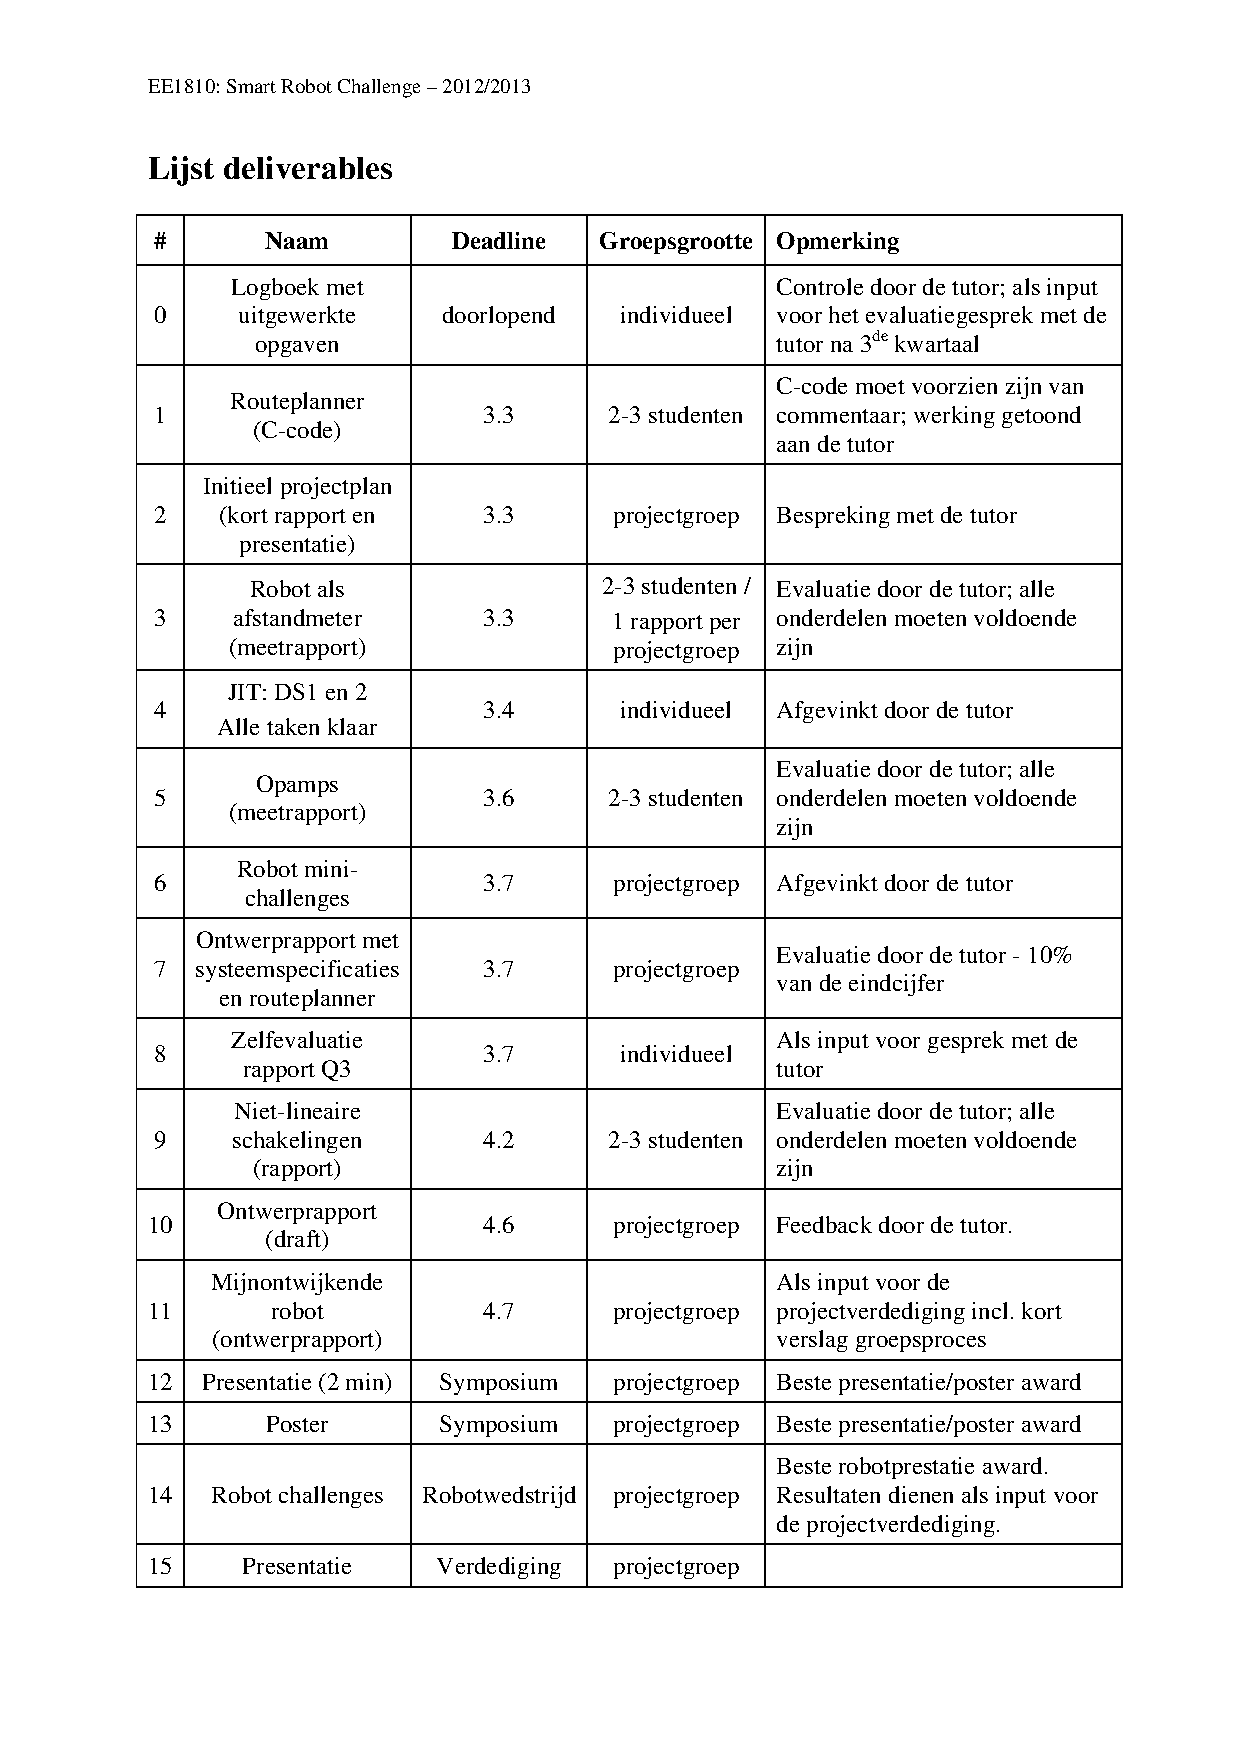
\includegraphics[scale=0.8]{deliverables-rc.pdf}

\end{document}

